Da die exakte Berechnung einer Kollision signifikant viel Rechenleistung benötigt, ist eine Vorfilterung sinnvoll. Diese schließt einen Großteil der Objektpaare schon vorher aus. Eine Kollision kann z.B. nur dann passieren, wenn die Hüllobjekte der beiden Objekte ebenfalls kollidieren (wegen der Eigenschaft $\mathcal{AABB}(AABB_o) \supseteq K_o$). Hier wird als Hüllobjekt eine AABB verwendet. Bestimmte Arten der logischen Kollision benötigen außerdem keine genauere Berechnung, sodass die verbleibenden Objektpaare nach der Vorfilterung direkt eine logische Kollision eingehen. Um verschiedene Arten der Kollision behandeln zu können und die Objektpaare dem richtigen Algorithmus für die nächste Stufe zuführen zu können, wurde im Rahmen des Projekts eine Komponente erstellt, die dieses Problem mit austauschbarem Vorfilterungsalgorithmus löst. (Ungenügende Ansätze der Behandlung verschiedener Kollisionstypen unter Verwendung eines nicht austauschbaren Vorfilterungsalgorithmus haben schon vor dem Projektstart in der Codebasis existiert). \\
Logische und physikalische Kollisionen werden als (lokale) Interaktionen zusammengefasst und werden in 2 Kategorien eingeteilt:
\begin{enumerate}
\item Symmetrische Interaktionen:\\
Beide Objekte des Objektpaares gehören der selben Klasse an (z.B: die Kollision rigider Objekte, wie sie in Abschnitt~\ref{sec:l2} beschrieben wird).
\item Asymmetrische Interaktionen:\\
Objektpaare setzen sich aus 2 Objekten verschiedener Klassen zusammen (z.B. Projektil und treffbares Objekt). Kollisionen innerhalb der selben Klasse treten hier nicht auf (Projektile interagieren nicht mit anderen Projektilen).
\end{enumerate}

In jeder Kategorie können mehrere Interaktionstypen enthalten sein. Jeder Typ wird hier einzeln betrachtet und ihm kann so ein eigener Vorfilterungsalgorithmus zugewiesen werden, der entsprechend zugeschnitten und problemspezifisch optimiert werden kann.
Die Aufgabe des Vorfilterungsalgorithmus unterscheidet sich je nach Kategorie der Interaktion etwas:
\begin{enumerate}
\item Symmetrische Interaktionen: Aus Menge aus n Objekten werden alle diejenigen //TODO Mathe Format (maximal n²) Objektpaare ausgewählt, deren AABBs sich überschneiden (ein beliebiges der beiden Objekte muss dann über die Interaktion mit dem Partner informiert werden). Als untere Schranke kann man Omega(n+i) angeben, wobei i die Anzahl der tatsächlichen Überschneidungen ist. Die obere Schranke O(n²) erhält man durch naives Ausprobieren jeder Kombination.
\item Asymmetrische Interaktionen: Aus 2 Mengen von m und s Objekten werden alle diejenigen Objektpaare mit jeweils einem Mitglied aus jeder Menge ausgewählt, deren AABBs sich überschneiden (das Objekt der Master-Klasse muss dann über seine Inkteraktion mit dem Partner aus der Slave-Klasse informiert werden). Als untere Schranke kann man Omega(m+s+i) angeben. Die obere Schranke O(m*s) erhält man durch naives Ausprobieren jeder Kombination.
\end{enumerate}

Für die Laufzeit bei praktischen Problemen sei angemerkt, dass die Konstante oft eben so wichtig zu betrachten ist wie die asymptotische Komplexität. \\

Im folgenden werden 2 Algorithmen, die im Rahmen des Projekts implementiert wurden, näher beschrieben.

//TODO format
1. Boxsort
//TODO
Bei Boxsort //TODO litref wird eine binäre Baumstruktur aufgebaut, in der anschließend nach einem Raumbereich (einer AABB, der query box QB) gesucht werden kann, sodass alle damit überlappenden einsortierten AABBs gefunden werden. Aufgrund der Mehrdimensionalität und dem Einsortieren von Bereichen statt Punkten müssen erhebliche Änderungen an der Baum-Datenstruktur vorgenommen werden.\\
Ein Knoten enthält genau eine einsortierte AABB. Als Sortierschlüssel wird dort das niedrige Ende der einsortierten AABB in einer bestimmten Dimension gewählt, es gilt also //TODO Mathe key aus S. Ist das obere Ende der QB in dieser Dimension kleiner als der Schlüssel, kann die höhere Baumhälfte ausgeschlossen werden und muss nicht mehr durchsucht werden. Die Sortierdimension ist hier für jeden Knoten individuell wählbar.\\
Um die untere Baumhälfte ausschließen zu können, müssen jedoch weitere Informationen vorliegen. Da die maximale Ausdehnung nach oben in der vorher festgelegten Koordinate nicht durch den Knoten festgelegt werden kann, muss jeder Knoten, der darunter liegt, berücksichtigt werden und der Maximalwert aller ermittelt werden. Dieser wird nach vollständigem Baumaufbau dann im Knoten vermerkt.\\
Wird zu beiden Teilbäumen auch der jeweils andere Extremwert gespeichert, entsteht eine 1-Dimensionale AABB und beide Teilbäume können identisch behandelt werden. Dann kann für jeden individuell ein Überlappungstest bestimmen, ob sich QB mit dem Teilbaum überschneidet. So können unter bestimmten Umständen sogar beide Teilbäume ausgeschlossen werden. Ein Beispiel dafür sieht man in Abb.~\ref{fig:boxsortNode}.\\

\begin{figure}
    \centering
    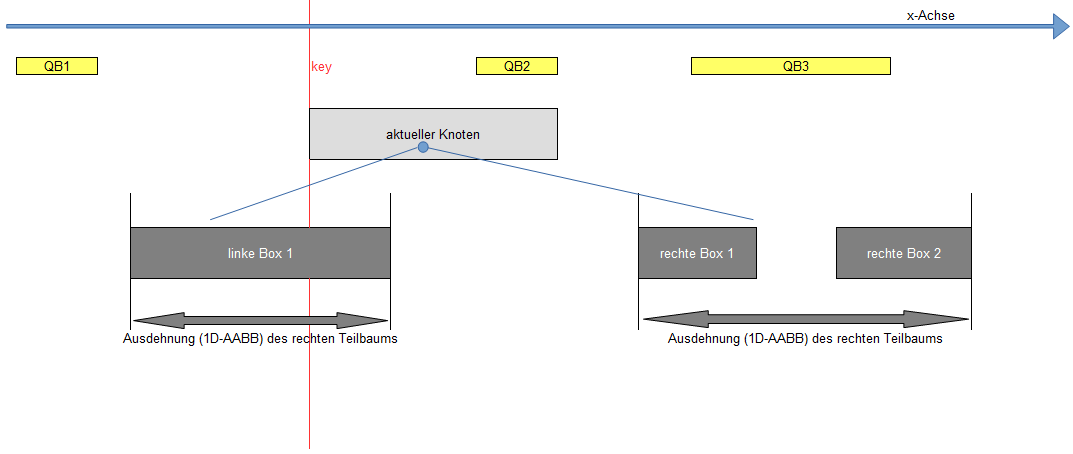
\includegraphics[width=0.5\textwidth]{./res/BoxsortNode.png}
    \caption{2D-Beispiel für einen Knoten im Suchbaum. Relevant für die Sortierung ist bei diesem Knoten die x-Achse. Die Teilbäume werden nicht gezeigt, die darin enthaltenen AABBs werden in dunkelgrau nebeneinander dargestellt. Query Boxes sind oben in gelb dargestellt.}
    \label{fig:boxsortNode}
\end{figure}

Man sieht in Abb.~\ref{fig:boxsortNode}, dass QB1 sich komplett links der Bereiche der beiden Teilbäume befindet. Der Suchlauf endet für QB1 somit direkt bei dem dargestellten Knoten. Auch QB2 überschneidet sich mit keinem Bereich der Teilbäume, aber der Grund dafür ist diesmal die Lage in der Mitte von beiden. Solch eine Lage muss im Allgemeinen nicht zwangsläufig existieren, denn die Bereiche der beiden Teilbäume können auch überlappen. QB3 hingegen überlappt mit dem rechten Teilbaum. Für die Suche scheidet also nur der linke Teilbaum aus. Sie wird im rechten Teilbaum rekursiv fortgesetzt. Man kann auch query boxes konstruieren, sodass eine Überlappung mit beiden Teilbäumen auftritt. Dann muss die Suche in beiden rekursiv fortgesetzt werden.\\
Der eigentliche Sortiervorgang zum Aufbau des Baums findet mit einer modifizierten Quicksort-Variante statt. Dabei wird das Pivot-Element zum Knoten und die restlichen Elemente werden entsprechend des Schlüssels in den beiden Teilbäumen zugeteilt. Bei der Zuteilung wird nebenbei die 1D-AABB des Teilbaums ermittelt, indem die Ausdehnung bei jedem Zuteilungsschritt ggf. vergrößert wird, um das aktuelle Element zu berücksichtigen.\\
Als Heuristik für das Finden des Pivot-Elements wird der Median einer zufälligen Auswahl von bis zu 9 Elementen gewählt. Die Sortierdimension wird an der Wurzel auf die x-Achse festgelegt. Beim Einsortieren in die beiden Teilbäume wird eine Heuristik berechnet, die im jeweiligen Teilbaum die beste Sortierdimension abschätzt. Dafür wird für jede Dimension die durchschnittliche Größe der Objekte in dieser Dimension berechnet. Damit kann man die Dichte der Objekte in jeder Dimension abschätzen, wenn man den Gesamtbereich kennt, den die AABBs einnehmen. Gewählt wird die niedrigste Dichte.\\
Im Gegensatz zum in //TODO ref beschriebenen Spatial Hashing müssen für den Boxsort-Algorithmus vor dem Start erst alle Objekte gesammelt werden. Im asymmetrischen Fall muss dann entschieden werden, aus welcher Menge der Objekte der Baum aufgebaut wird. Für den Benutzer stehen hier mehrere Modi zur Verfügung. Zur Auswahl stehen unter anderem die Möglichkeiten, die Anzahl der Elemente je Menge zu vergleichen und die größere oder kleinere zu verwenden, um den Baum aufzubauen. Der Grund dafür wird deutlich, wenn die Laufzeit im erwarteten Fall betrachtet wird. Wenn die Menge M m Elemente und die Menge N n Elemente enthält und der Baum aus N aufgebaut wird, dann ist dafür $mthcal{O}(n*log(n))$ Zeit nötig. Wenn eine ausreichende Verteilung im Raum vorliegt und die Größe von QB in der selben Größenordnung sind wie Elemente aus N ist, dann benötigt die Suche $mthcal{O}(log(n))$ Zeit //TODO Zitat Boxsort abstract. Insgesamt wird also für das Finden aller Überlappungen $mthcal{O}(n*log(n)+m*log(n))$ Zeit benötigt. Anhand dieser Form würde man vermuten, dass die Wahl immer auf M als größere Menge fallen sollte. In der Praxis ist vor den Termen $n*log(n)$ und $m*log(n)$ aber ein Vorfaktor, der nicht identisch ist. Messungen ergaben einen nahezu konstanten Vorfaktor beim Baumaufbau. Für den Abfrage-Durchlauf ist der Faktor jedoch stark abhängig von der konkreten Verteilung der eingegebenen AABBs. Messungen ergeben einen um den Faktor von ca. 3 verschiedenen Vorfaktor unter stark idealisierten Bedingungen, einen nahezu identischen unter moderaten Bedingungen und einen ca. 3-mal größeren unter erschwerten Bedingungen (Durchschnittliche Kollisionen pro Objekt>3). Den Benchmark-Ergebnissen in //TODO ref kann man jedoch entnehmen, dass wenn die beiden Mengen die gleiche Verteilung aufweisen, die Auswahl der Menge auf die Performance keinen signifikanten Einfluss hat. Um trotzdem offen für zukünftige problemspezifische Erkenntnisse zu sein, bleibt die Option, die größere oder die kleinere Menge zu wählen. Dazu kann ein Präferenz-Faktor angegeben werden, der vor der Entscheidung mit der Anzahl der Master-Elemente multipliziert wird. Als weitere Modi kann der Benutzer einstellen, dass nur eine der beiden Mengen für den Baum verwendet werden darf. Dies wird für Fälle gebraucht, wo die o.g. Bedingungen für die Komplexität der Suche im Baum nur für eine der beiden Mengen zutreffen.\\
Im symmetrischen Fall wird jedes Objekt sowohl in den Baum einsortiert als auch als QB in dem Baum gesucht. Dabei muss die QB selbst aus den Ergebnissen wieder entfernt werden.\\

//TODO format
2. Spatial Hashing
Die Grundidee besteht hier dabei, den Raum in viele Bereiche (sog. chunks) aufzuteilen und Kollisionspaare nur innerhalb dieser Bereiche zu suchen. Sind 2 Objekte weit voneinander entfernt und somit nicht im selben chunk, ist eine Überschneidung der AABBs nicht möglich und muss deshalb auch nicht betrachtet werden. Ein Beispiel für 2 Dimensionen sieht man in Abb.~\ref{fig:spatialHashing}.

\begin{figure}
    \centering
    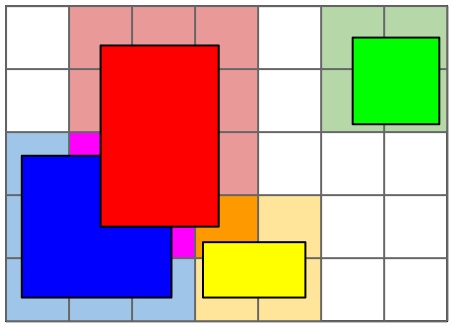
\includegraphics[width=0.5\textwidth]{./res/spatialHashingAABB.png}
    \caption{2D-Beispiel von Spatial Hashing von AABBs (stark gefärbte Rechtecke). Die leicht gefärbten Bereiche sind chunks, die ein Objekt der entsprechenden Farbe(n) beinhalten.}
    \label{fig:spatialHashing}
\end{figure}

Man sieht in Abb.~\ref{fig:spatialHashing}, dass Objekte mit mehreren chunks überlappen können. Ein Objekt muss sich in jedem chunk anmelden, das sich mit seiner AABB überschneidet, zu sehen z.B. beim grünen Objekt, das sich in den 4 chunks rechts oben anmelden muss. Gibt es keine weiteren Objekte in den chunks, wo sich das Objekt angemeldet hat, müssen keine potentiellen Kollisionen berechnet werden. Ist dies für alle Objekte der Fall, ist die optimale Komplexität O(n) im symmetrischen Fall erreicht (bei konstanter Maximalgröße von Objekten). Im asymmetrischen Fall können mehrere Objekte im selben chunk angemeldet sein, ohne dass eine Kollision auftritt, solange die Objekte alle vom selben Typ sind. In diesem Fall ist die optimale Komplexität von O(n+m) im asymmetrischen Fall erreicht (bei konstanter Maximalgröße von Objekten). \\
Werden mehrere Objekte, die für eine Kollision kompatibel sind, in einem chunk angemeldet, so müssen alle potentiellen Kollisionspaare überprüft werden (hier mit naivem //TODO Mathe O(n²) bzw. O(n*m) Algorithmus). Die Überprüfung kann entweder direkt bei der Anmeldung erfolgen (hier implementiert) oder erst nach Eintragung aller Objekte erfolgen, was die Auswahl an für die weitere Auflösung verwendbaren Algorithmen erhöht. \\
Ein potentielles Problem kann in Abb.~\ref{fig:spatialHashing} bei der Überschneidung des roten und blauen Objekts betrachtet werden. Erfolgt eine Überlappung in mehreren chunks, besteht die Gefahr der mehrfachen Behandlung von Kollisionen. Deshalb wird während der Partnerfindung ein Hashtable mit schon behandelten Objekten mitgeführt, womit effizient Duplikate vermieden werden. Auf diese Maßnahme kann verzichtet werden, wenn sich das Objekt nur in einem chunk befindet.\\
Um das Anlegen vieler leerer chunks zu vermeiden und trotzdem schnellen Zugriff zu haben, wird ein Hashtable zur Verwaltung der chunks verwendet. Dazu wurde eine passende Hashfunktion gesucht und eingebunden, die plattformunabhängig aber dennoch mit sehr geringer Laufzeit $HASH: \mathcal{I}^3 \mapsto \mathcal{I}_{64}$ mit $\mathcal{I}_{64}$ als 64-Bit Integer einem Hashwert zuordnet. $i: (i, f)\in\mathcal{S}$
//TODO mathe gedöhns richtig machen
Der Idealfall für Spatial Hashing, wo es asymptotisch optimal wird, wurde oben schon beschrieben, in der Paxis tritt dies jedoch nur selten auf. Problematisch können dort z.B. große Objekte werden, denn die Anzahl chunks, wo eine Anmeldung erforderlich ist, und damit die Laufzeit, steigt dann linear mit dem Volumen. Ein weiterer Problemfall ist, wenn zu viele Objekte in einem chunk sind. Denn selbst wenn sie sich nicht überschneiden, ist dann eine //TODO O(n²) bzw. O(n*m) Auflösung erforderlich (n und m hier Anzahl Objekte im chunk). Ob dieser Algorithmus für den Einsatz sinnvoll ist, hängt also davon ab, ob diese Probleme bei dem bestimmten Interaktionstyp auftreten, wo er eingesetzt werden soll. \\
3. Vergleich der Verfahren
Um die Performance der Algorithmen bei verschiedenen Szenarien objektiv bewerten zu können, wurde im Rahmen des Projektes eine Benchmark-Umgebung implementiert. Getestet wurden verschiedene Szenarien mit verschiedenen Parametern. Gemeinsam haben alle Szenarien die Testparameter Problemgröße (Objektzahl) und absolute Größe der Objekte (aus $\mathcal{S}$).\\
Das Standardszenario ist eine Gleichverteilung von Objekten im Raum. Ein zusätzlicher Testparameter hier ist die Dichte der Objekte, welche das Verhältnis der Durchschnittsgröße (längste Ausdehnung in einer Achse) zur Durchschnittsdistanz (der Mittelpunkte) darstellt. Die asymmetrische Variante hat zusätzlich noch das Verhältnis der Menge an Objekten beider Klassen als Testparameter.\\
Ein weiteres rein asymmetrisches Szenario "Shotgun" modelliert eine Menge an Projektilen und Zielen. Die Ziele sind weiterhin gleichverteilt, die Projektile modellieren jedoch eine Schrotladung, bei der viele Projektile gemeinsam fliegen. Dies bedeutet, dass die AABBs sich weitgehend überlappen aber alle nur in einem Teilbereich erzeugt werden, der nicht dem Erzeugungsbereich der Ziele entspricht. Ein Testparameter beschreibt die erwartete Anzahl Ziele im Erzeugungsbereich der Projektile. Das Verhältnis zwische Zielen und Projektilen ist ein weiterer Parameter.
